\section{Project objectives}\label{sect_objective}
In this section, we briefly discuss the project and its objectives.
\begin{figure}[H]
	\begin{center}
		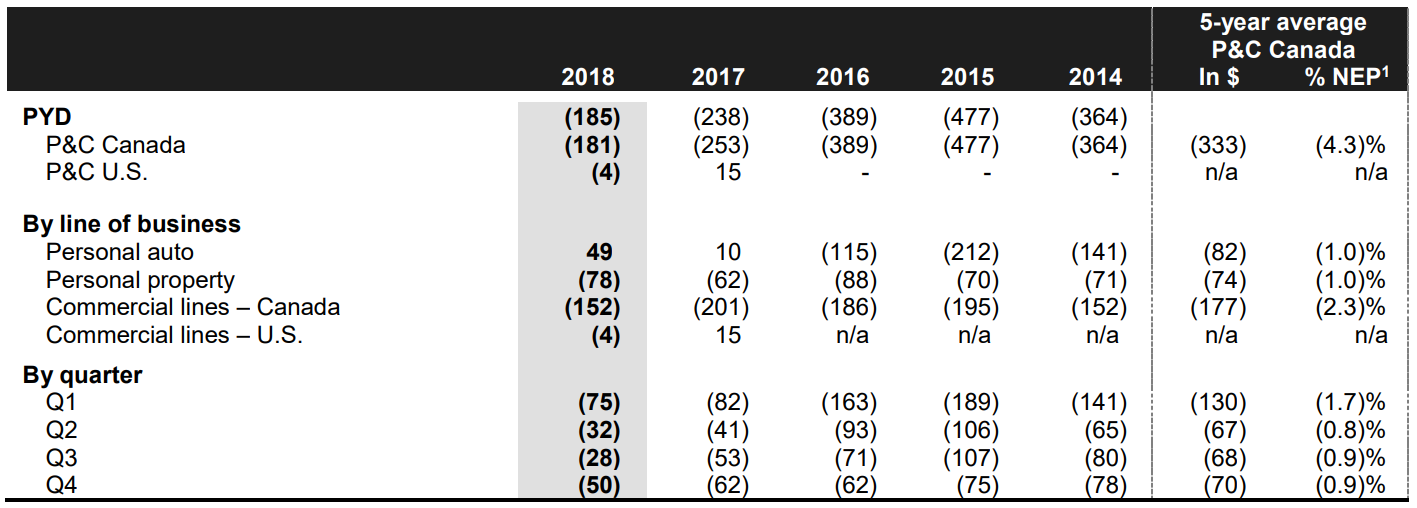
\includegraphics[scale=0.4]{Graphiques/PYD} 
		\renewcommand{\figurename}{Figure}
		\caption{Unfavourable (favourable) prior year development, \cite{intact2018}}\label{Ill_annual_report}
	\end{center}
\end{figure}
The IBNR project arises from the results of \cite{intact2018} annual report, see figure \ref{Ill_annual_report}. The prior year development (PYD) of the Personal auto line is at 49 million of which 20 million are auto physical damage. PYD represents the change in total prior year claims liabilities during a specific period, in this case 2018. An increase in claims liabilities is referred to as an unfavourable prior year development. This means that the actuarial department underestimated the claim losses by 49 million. Even if percentage-wise this is not very significant, it still is a large amount for a line of business, which should not be fluctuating as much. Such unfavourable development is not desirable and therefore Intact's higher management launched an investigation regarding the origin of this issue. They decided that the claims team should investigate the issue and develop a new model which should exist in parallel with the model of the actuarial department. This project started in summer 2019, while I got involved by autumn 2019. \\ 
The idea is to have a second model which allows the actuarial department to assess if their model works correctly. If both models converge, they can have more confidence in their booked numbers. If the discrepancies are too large, it will trigger further investigation. It is important to note that the booked PYD is shown in the Intact annual reports and is often used by investors to determine Intact's performance. In addition, the actuarial department wants a model which is interpretable and comprehensive. At this stage, a black box model is not a solution, since it does not allow an exact understanding of the results.\\
The model uses historical claims data in order to predict the incurred but not reported (IBNR) personal auto claims for a specific month. The actuarial department uses an advanced chain-ladder approach. We were asked to find a different method which we discuss in more detail in section \ref{Sect_Methodologie}. Consequently, the main objective of this project is:
\begin{center}\emph{
		develop a model which outperforms the current model used for booking the PYD. This model has be interpretable and dynamic enought to be able of capturing recent data changes.
}\end{center}
Before diving into the model itself, we have to fully understand the data used for the predictions. Thus, in the next section, we analyze the data we use for the model.

 

	
	